
\chapter{Implementation Dataset Creator application}
The CV.ILIBG expects that developers have a model for detecting objects that can be used by the inference engine utilized by the Android library. The subject of this thesis is not to provide a way to gather these raw image data, let alone labeled data, for training these models. However, it provides an application that aims to simplify this problem.

This chapter will explain the implementation and design choices for the CV.ILIBG \textbf{Dataset Creator} a desktop application that focuses on labeling image data, enhancing the data with synthetic data generation, saving and exporting these datasets in a format that is ready to be used for training, and lastly, lightweight training of these models within the application.

% ===========================================================================================

% ===========================================================================================


\section{Design choices for the desktop application}
The \textbf{Dataset Creator} should be an application and a tool that can be used by developers on all operating systems, as Android development is not exclusive to a single operating system. Therefore, it is necessary to use multi-platform frameworks. Also, while the application is part of this thesis, it should be usable without the mobile library for developers who might want to use it as an annotation/labeling tool or for creating synthetic data. Therefore, all metadata about the saved datasets must be saved in one of the standard formats, allowing users of the application to convert datasets into other formats using external tools, should they desire to.

\subsection{Language for developing \textbf{Dataset Creator}}
There are plenty of options for choosing a library or framework that supports desktop development. Most of these languages support multi-platform development. However, some of them, like C++ would require multiple binaries or building from source. On the other hand, interpreted languages such as Java provide seamless multi-platform deployment, and the code from the mobile applications could be shared with the desktop dataset application. 

However, while Java has many positives, it is also known to be a verbose language with more code overhead. Python, on the other hand, seems to be more popular for neural networks and object detection in general. Should the use case of this application require raw computational performance, a different language such as C++ or Java, which are generally faster than Python \footnote{Java versus Python performance benchmarks on PlanningAI models: \url{https://timefold.ai/blog/java-vs-python-speed\#so-how-fast-is-timefold-solver-for-python}}. However, as the main purpose of this application is to be usable and provide nimble multi-platform development, Python is preferred for this task. 

\subsection{Choosing library or framework for desktop development}
Many modern frameworks support multi-platform development. The list became a bit narrower by choosing Python as the main language. Options such as Kivy, Tkinter, PyQt, PySide, Flet, and many more could be found as fully fledged development frameworks; some of them even support mobile development. Qt is a cross-platform application development framework for desktop, embedded, and mobile applications \cite{qt}. It is supported and used by many companies; however, it was chosen mainly because I, as the author, have previous experience with this framework, which allowed smoother and faster development of the application.

However, for Python, there are two versions of Qt: PyQt and PySide. These two versions of Qt for Python are very similar nowadays, and the main difference comes from who manages the projects. PyQt is managed by Riverbank Computing Ltd.\footnote{\url{https://www.riverbankcomputing.com/software/pyqt/intro}}, while PySide is managed and maintained by The Qt Company \footnote{\url{https://doc.qt.io/qtforpython-6/}}. The most notable difference is licensing. PyQt is available under GPL or commercial license, while PySide uses a more permissive LGPL license \footnote{\url{https://www.pythonguis.com/faq/pyqt6-vs-pyside6/\#licensing}}. While this project will be open and not used for commercial purposes, the more permissive license is a positive. Therefore, PySide was chosen as the framework for desktop development.

\subsection{Creating user interface}
The first iterations of the application used hard coded user interface elements (from here on referred to as UI). However, code like this was hard to navigate and manage. Because of that, a \textbf{QtDesigner}, a tool from Qt that allows developers to create windows and widgets used by the application with a graphical user interface, was introduced. 

\begin{figure}[hbt]
	\centering
	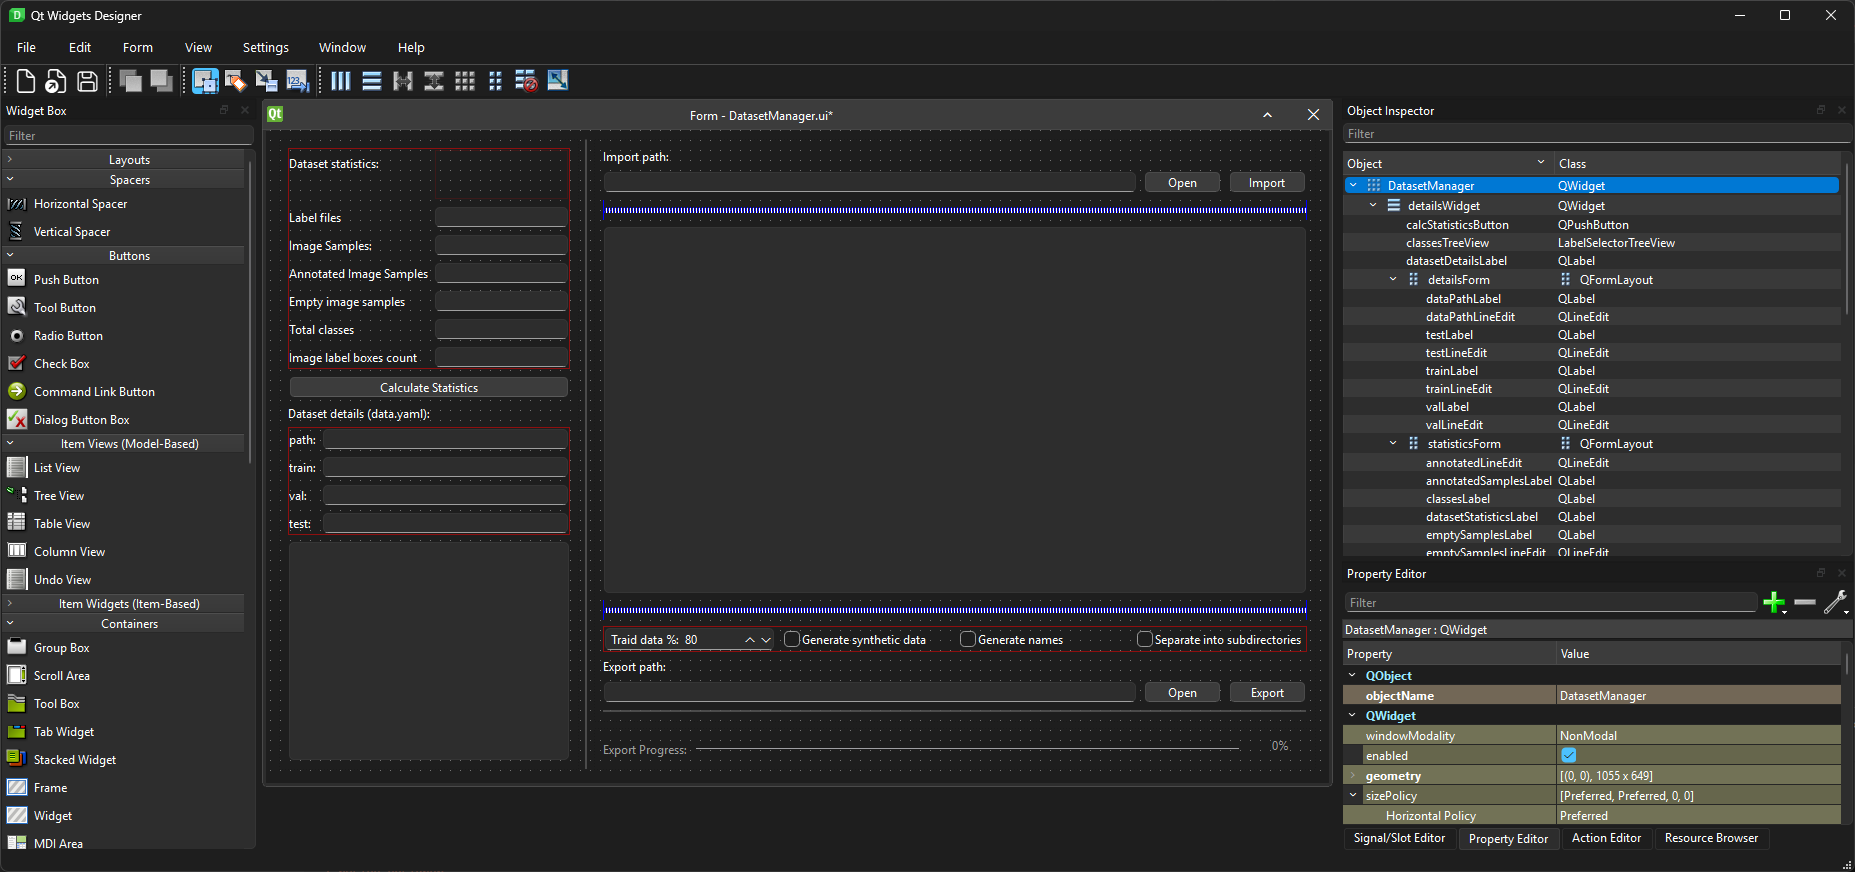
\includegraphics[width=0.80\textwidth]{obrazky-figures/qtdesigner_screenshot.png}
	\caption{Screenshot from the QtDesigner application}
	\label{QtDesignerScreenShot}
\end{figure}

The output of the \textbf{QtDesigner} are \texttt{.ui} files. These files can be loaded dynamically using \texttt{QUiLoader} or compiled into Python files. Dynamically loading files is easier as it does not require recompiling files after each change in the UI. However, using this method, VSCode loses the ability to provide static checking, as provided by the PyLance extension used for cleaner and less error prone code. Therefore, the other approach was chosen, and the project contains \texttt{.ui} and compiled \texttt{.py} files that contain the UI elements. These are loaded into the widgets, each hosting different functionality. 


% ===========================================================================================

% ===========================================================================================

\section{Managing the datasets}

The rest of this chapter focuses on each page that provides different functionality. This page hosts actions related to importing and exporting image datasets. It also contains the general dataset information in YOLO format that uses the \texttt{data.yaml}.

\begin{figure}[hbt]
	\centering
	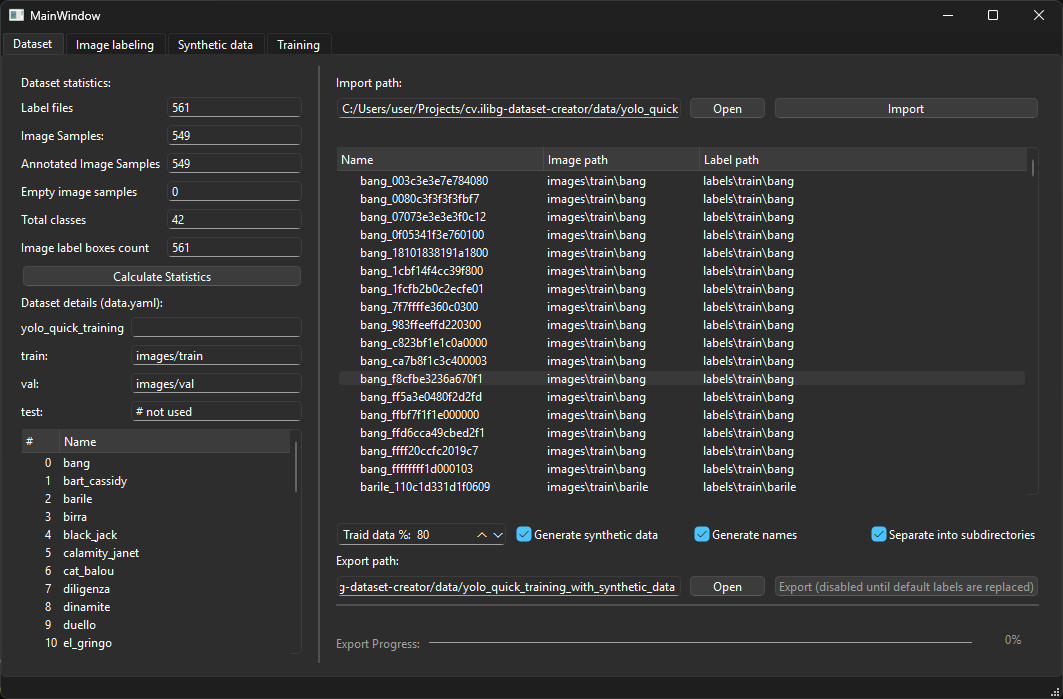
\includegraphics[width=0.70\textwidth]{obrazky-figures/datasetManager_screenshot.png}
	\caption[Data Creator screenshot - Dataset loading]{Screenshot from the Dataset Creator, page for managing datasets.}
	\label{DatasetManagerScreenShot}
\end{figure}

\subsection{Importing dataset}
Imported data will be gathered from the root of the folder and recursively searched for all image files (\texttt{.png} and \texttt{.jpg} extensions), text files containing annotations, and a single \texttt{data.yaml} file. Image data should be paired with text data that have the \texttt{.txt} extension; both files must have the same name for the importer to recognize them as an image data and label data pair. These files can be in separate directories, and multiple image data can have the same name. However, multiple text data cannot be loaded, as it would be ambiguous to which image data the text data belongs. 

Imported image and label data are shown in \texttt{QTreeView} in the format: image name, path to the image, and label path. The format is shown in the middle part of Figure~\ref{DatasetManagerScreenShot}.

Datasets that use the Ultralytics YOLO format \footnote{Object Detection Datasets Overview: \url{https://docs.ultralytics.com/datasets/detect/\#ultralytics-yolo-format}} or have already been exported by the application will contain a \texttt{data.yaml} file that includes the paths to training and validation data, as well as the object class values paired with string values. These pairs are also used by the \textbf{Dataset Creator} tool to show the names of the classes instead of their numerical representation. Values inside the \texttt{data.yaml} can also be changed within the application. However, it is recommended to use the default values. It is also possible to rename classes; however, changing their index is not supported.

% ===========================================================================================

\subsection{Exporting datasets}
\textbf{Exporting} is another part of the dataset tab. The whole dataset with annotated data is exported to the specified path in the format used by the Ultralytics YOLO datasets. While exporting, the application provides different options: 

\bigskip
\begin{itemize}
  \item {\textbf{Training data percentage} will set the amount of data in integer percentage that will be used for training; the rest will be used for validation.}
  
  \item {\textbf{Generate name from the class} will replace images and text label names with \texttt{classname\_hash}, where the classname is the detected class, and hash is an image data hashed into the 16 character string. Images with multiple classes will be named \texttt{mixed\_hash}.}
  
  \item {\textbf{Separate classes into subdirectories} will sort the images and labels based on their detected class into subdirectories. Images with multiple classes will be put into mixed subdirectory.}
  
  \item {\textbf{Generate synthetic data} enables generating of synthetic data.}
\end{itemize}
\bigskip

% ===========================================================================================

% ===========================================================================================


\section{Labeling/image annotation}
This page is separated into 4 different sections. All of the sections manipulate the images or labels/annotations for those images.

\begin{figure}[hbt]
	\centering
	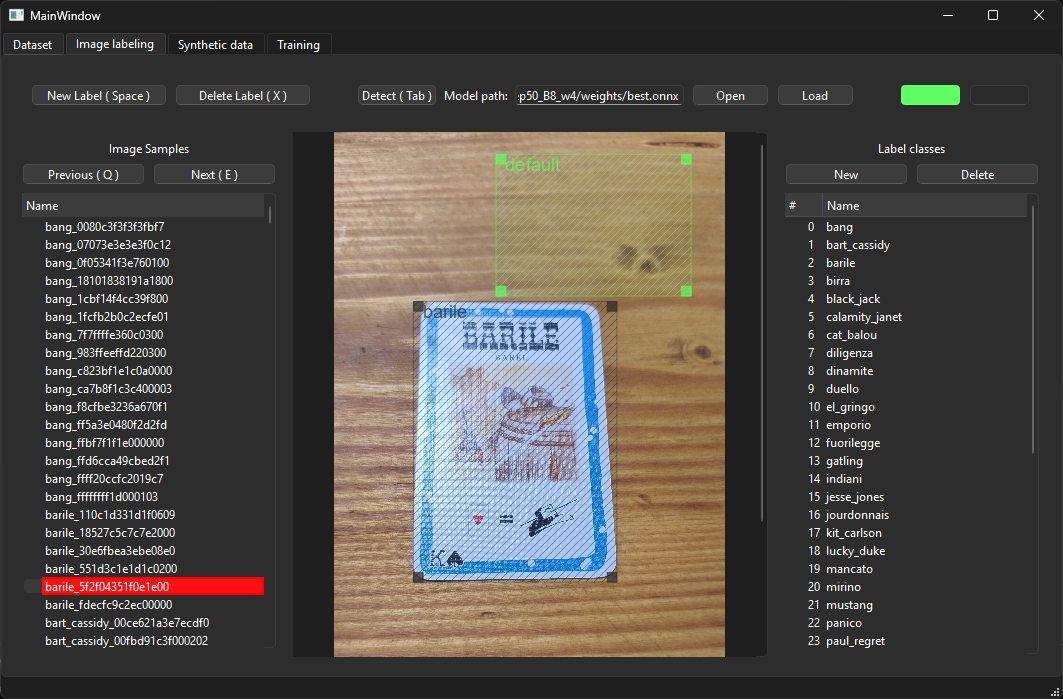
\includegraphics[width=0.70\textwidth]{obrazky-figures/dataLabeler_screenshot.png}
	\caption[Data Creator screenshot - Labeling]{Screenshot from the Dataset Creator, page for annotating/labeling image data.}
	\label{DataLabelerScreenShot}
\end{figure}

\subsection{Image label boxes for annotating the image data}
Annotating or labeling image data is done by creating rectangle bounding box-like objects on top of the shown image. These objects are called \texttt{ImageLabelBoxes} and are used for representing the annotated data in the application. Creating a box can be done by clicking \textbf{New label} or by pressing the keyboard shortcut \textit{"Space"}. These boxes can be moved and resized. 

If there are multiple \texttt{ImageLabelBoxes}, one of them will always be selected, and the others will be unselected. All actions can be performed only on the selected boxes. The colors that represent selected and unselected boxes can be changed with color pickers in the top right corner of the window.

Newly created boxes have a \textit{default} value. The \texttt{ImageLabelBoxes} with the \textit{default} value cannot be saved, and users will be warned with a red background in the \texttt{ImageSampleTreeView}. Deleting selected boxes is done by pressing the \textbf{Delete label} or by pressing the \textit{"X"} shortcut on the keyboard.

\subsection{ImageSampleTreeView}
\texttt{ImageSampleTreeView} is located on the left side of the page. Its purpose is to switch between the loaded images, also called image samples, which in code are represented by the \texttt{ImageSample} class. Switching can be done by clicking on the image sample, using the \textbf{Next} and \textbf{Previous} buttons, or by using the keyboard shortcuts \textit{"Q"} and \textit{"E"}.

\subsection{Label classes}
On the right side of the page is a \texttt{LabelSelectorTreeView} that contains all loaded classes. This view contains the index \textit{"\#"} of the label and its name. Both of these values are stored in the \texttt{data.yaml} file. Single clicking on one of the elements from the tree view will change the currently selected \texttt{ImageLabelBox}'s label to the clicked one. Double-clicking on the labels enables the editing mode in which the user can edit the name of the label. The index of the labels cannot be changed. These labels can be added and deleted using the \textbf{New} and \textbf{Delete} buttons. Deleting one label will update the indexes of all other labels with a higher index to move down.

\subsection{Automatic detection}
This page of the \textbf{Dataset Creator} contains the automatic object detection functionality. All the controls are located in the top section of the page. Models must be opened by providing a path or using the \textbf{Open} button, which will launch the operating system explorer. The \textbf{Load} button will load the model. After the model is successfully loaded, the \textbf{Detect} button will be enabled. The \textbf{Detect} button will try to detect objects in the current \texttt{ImageSample}. Automatic detection does not account for already created \texttt{ImageLabelBoxes} in the image sample. The automatic detection can also be activated with the \textit{"Tab"} key shortcut.  

The current version of the \textbf{Dataset Creator} supports only ONNX Runtime models for YOLO versions 8 to 11. This behavior can be changed by replacing the detector-like class  \texttt{ONNXDetector}.


% ===========================================================================================

% ===========================================================================================


\section{Synthetic data generation}
As mentioned before \ref{dataAugmentation} \textbf{overfitting} can be problem, especially for small datasets, because of that, \textbf{Dataset Creator} supports creating a synthetic data for trained models.

The synthetic data are only applied during the export process. Therefore, this page does not generate synthetic data; instead, it provides a way to create and edit filters that are used for synthetic data creation. For an explanation of data augmentation and synthetic data, see \ref{dataAugmentation}. 

\begin{figure}[hbt]
	\centering
	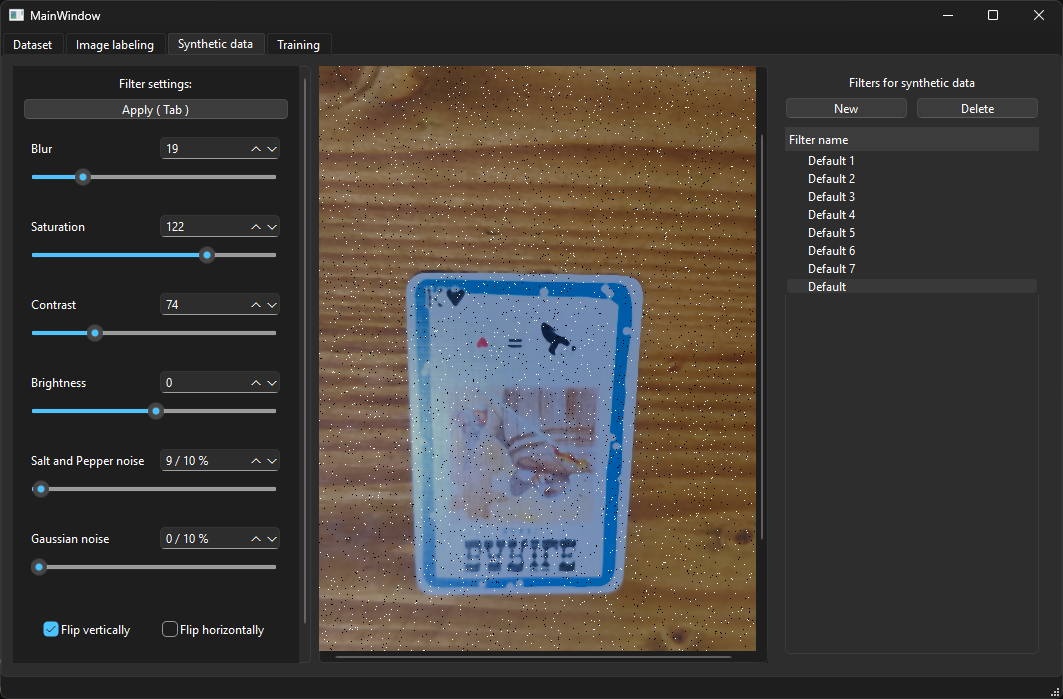
\includegraphics[width=0.70\textwidth]{obrazky-figures/synetheticDataEditor_screenshot.png}
	\caption[Data Creator screenshot - Synthetic data]{Screenshot from the Dataset Creator, page for editing filters applied to synthetic data.}
	\label{SynetheticDataEditorScreenShot}
\end{figure}

The middle of the page shows a preview of the filter. If the user did select any image sample in the \textbf{Image labeling} tab, no preview will be shown. 

On the top left side, there are individual settings that change the behavior of the current filter. Currently, the \textbf{Dataset Creator} supports these filters: Blur, Saturation, Contrast, Brightness, Vertical and Horizontal flip, Salt and Pepper, and Gaussian noise.

On the right side of the page is located \texttt{FilterPresetTreeView} that shows the current filters used by the dataset. These filters can be created or deleted using the \textbf{New} and \textbf{Delete} buttons. Filters can also be double clicked to change the filter's name. These filters are stored in the user settings; therefore, they are movable between projects/datasets.

It should be noted that the synthetic data will be exported as finished images with annotated data. This means that the additional data will take up more space. However, this format allows datasets to be used outside of the \textbf{Dataset Creator} and also results in faster training, as the data will not have to be augmented in memory during training.

\subsection{Options for synthetic data generation}

\begin{figure}[hbt]
	\centering
	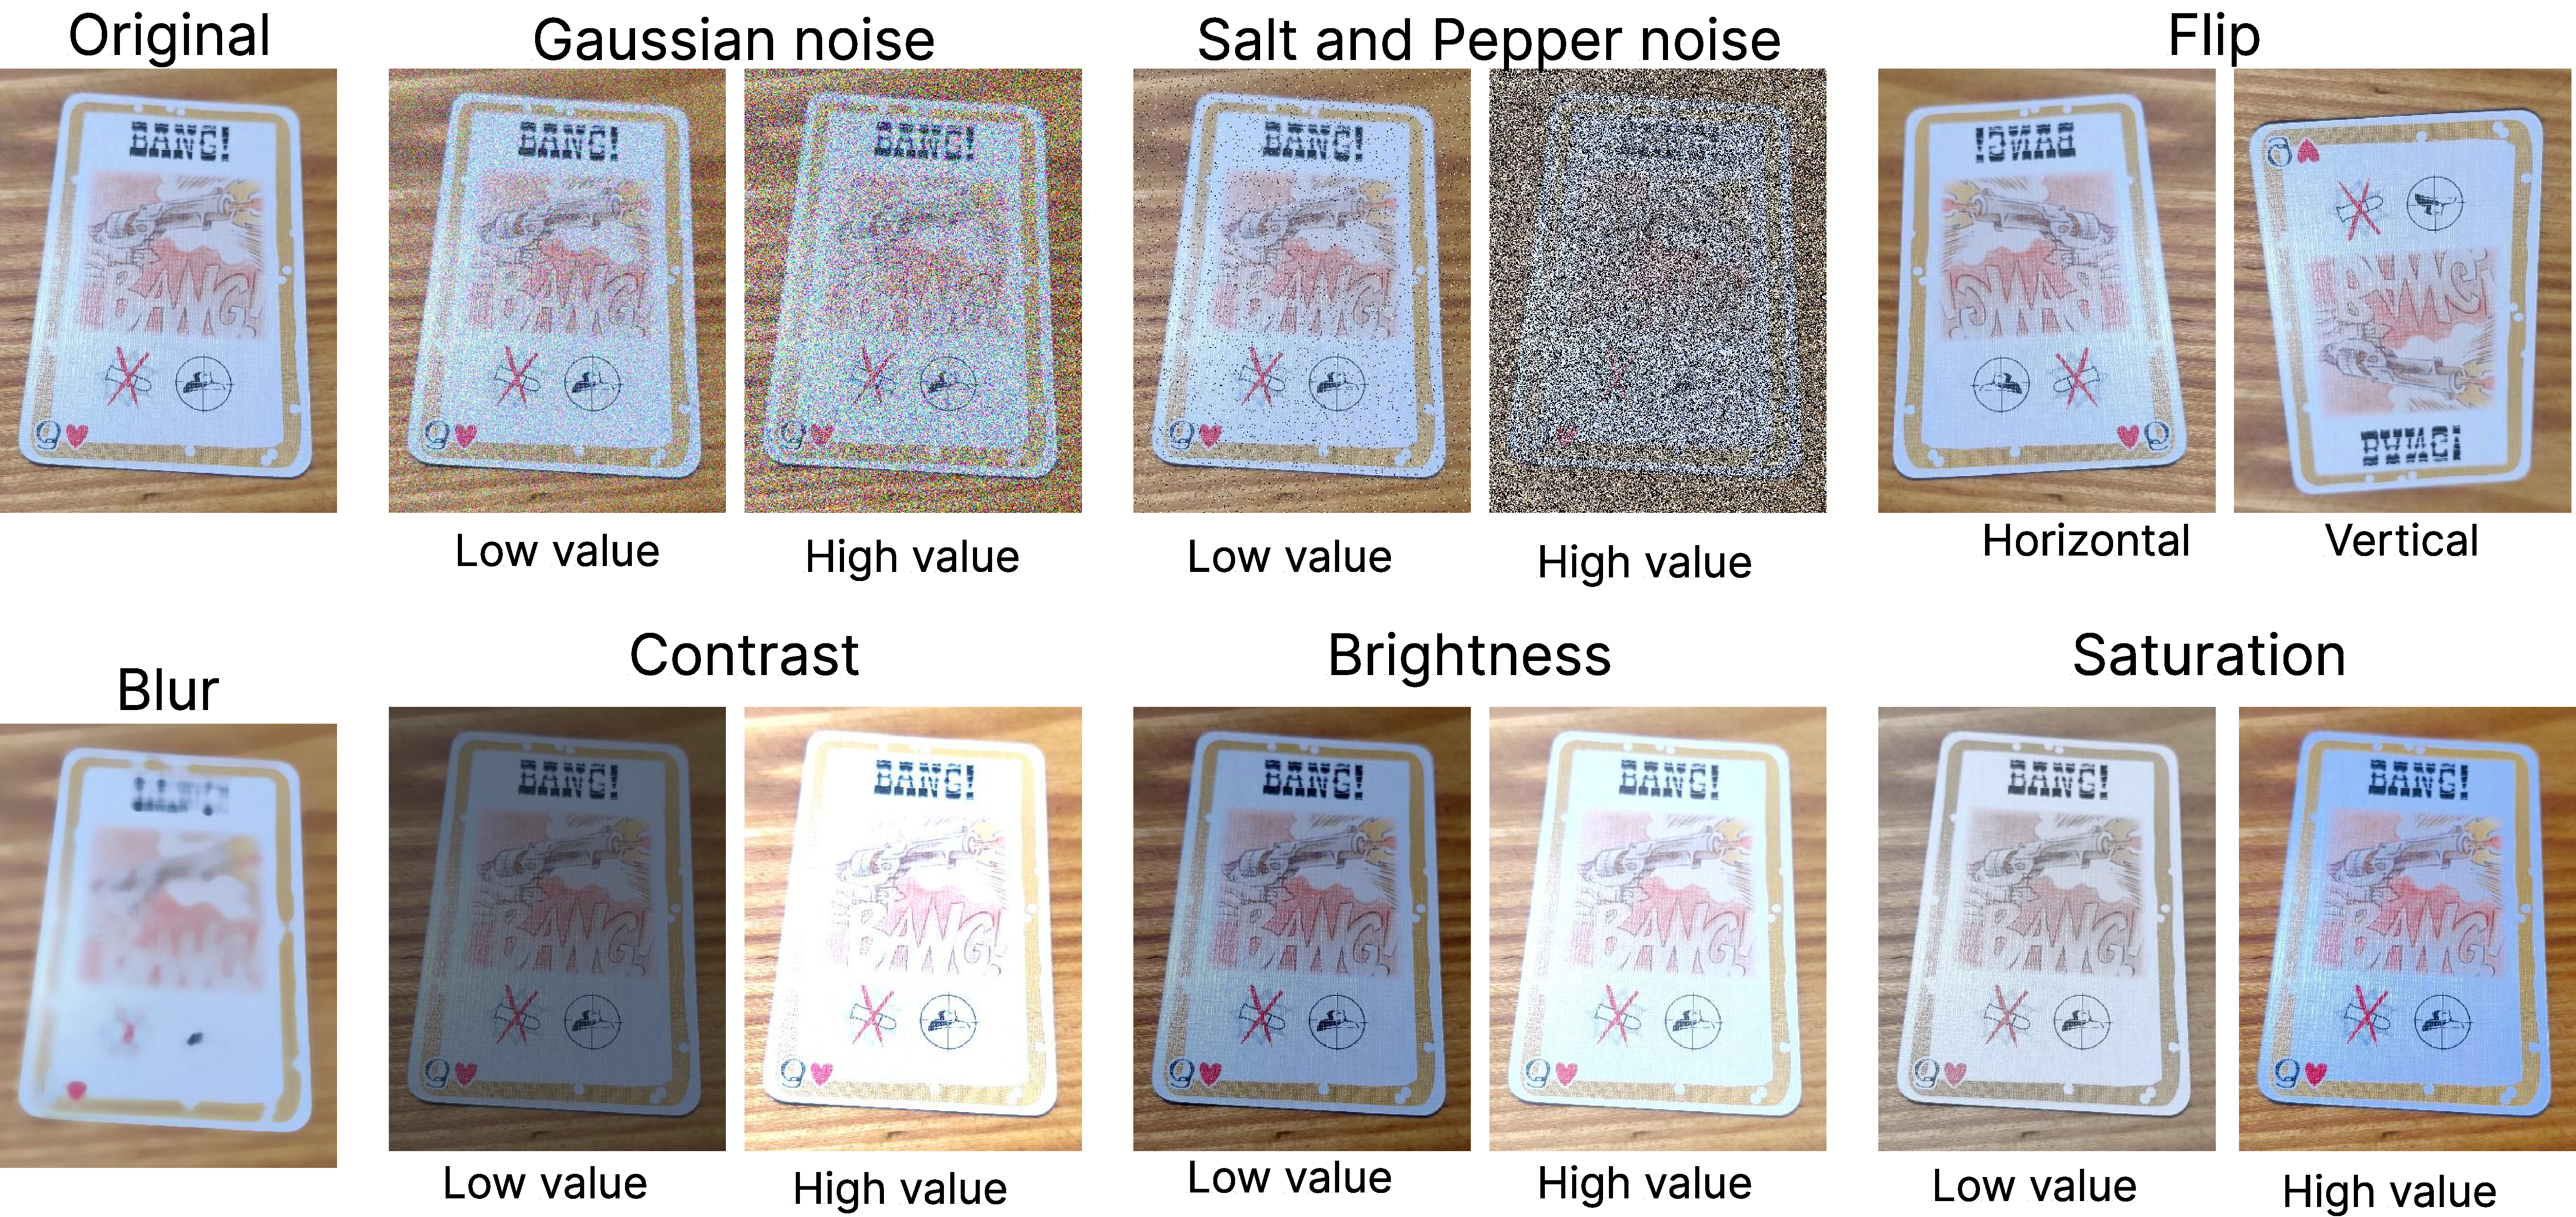
\includegraphics[width=0.95\textwidth]{obrazky-figures/synthetic_data_filters.pdf}
	\caption{Different values for synthetic data creation from the Data Creator application.}
	\label{SyntheticDataFilters}
\end{figure}

\textbf{Flipping}, as stated in \cite{dataAugmentation1}, is one of the easiest and most intuitive ways to augment the data. Simple vertical and horizontal flipping of images can create three additional images for training. However, using this method for data that contains direction sensitive \cite{dataAugmentation1} data such as letters and numbers might result in inaccurate labels.

\textbf{Blur} is also considered a good addition, especially as it removes noise from images that could be introduced by compression methods or from the camera itself.

The photometric transformations, such as \textbf{Saturation}, \textbf{Brightness}, and \textbf{Contrast}, can be used to change the representation of colors in image data, instead of the position of pixels. Lighting biases are an ongoing problem for object detection tasks; being able to artificially create darker or lighter images in a few steps can help enhance the neural network's adaptability \cite{dataAugmentation2}. Another example would be using saturation to accommodate different types of cameras in smartphones, as not all camera sensors are the same.

\textbf{Noise insertion} consists of injecting or changing pixel values in an image. This method is a very good solution for positional biases \cite{dataAugmentation2}. This method makes neural networks more robust, as real world data is not always perfect and often contains graphical artifacts \cite{dataAugmentation1}. The most common methods are \textbf{Gaussian} and \textbf{Speckle} methods. The \textbf{Gaussian} method is an additive technique that changes the original pixel value by adding or subtracting a value from it. \textbf{Speckle}, also known as Salt and Pepper, is a spike noise method. It changes pixels to their extremes, either white or black, reminiscent of salt and pepper.



% ===========================================================================================

% ===========================================================================================

\section{Training models in Dataset Creator}
The training page of the \textbf{Dataset Creator} is a simple training solution for developers who do not have access to a high performance server or who do not know how to use training algorithms. This page is supposed to be an easy, few click solution for users who want to train labeled data inside the \textbf{Dataset Creator}. Therefore, the settings available are the most crucial ones. Therefore, for more efficient model training, the developers should seek different solutions.

\begin{figure}[hbt]
	\centering
	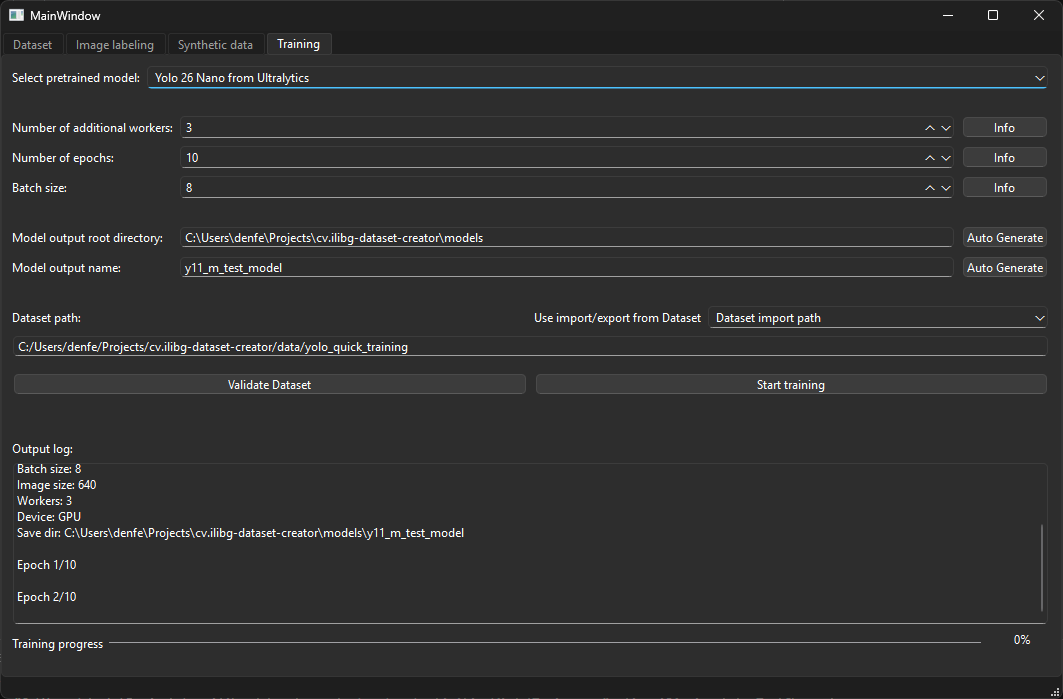
\includegraphics[width=0.70\textwidth]{obrazky-figures/modelTrainer_screenshot.png}
	\caption[Data Creator screenshot - Training]{Screenshot from the Dataset Creator, page for training models in application.}
	\label{ModelTrainerScreenshot}
\end{figure}

On top of the page is a model selection option for choosing different types of pretrained models that are used as the main body of the model. These models are then "re-trained" with a custom \textbf{head} that recognizes the classes defined in the dataset, see \ref{datasetCreatorUltralytics}.  

Available pre-trained models are Ultralytics' YOLO 8, 11, and 26 versions. Each YOLO version also contains two model sizes: \textit{Nano} and \textit{Medium}. These sizes represent the size of the model, with \textit{Medium} being more accurate but slower than \textit{Nano}. 

\bigskip
\begin{itemize}
  \item {\textbf{Epochs} is the number of training/validation steps that will be executed.}
  \item {\textbf{Workers} represent the number of additional workers that will be used during training. This value depends on the hardware capabilities of the machine running the application.}
  \item {\textbf{Batch size} represents the number of training examples in one training pass. Higher values mean higher memory use.}
\end{itemize}
\bigskip

Tested and preferred values with detailed descriptions for the Bang! demonstration application can be found in \ref{bangTrainingExperiments}. 

The next settings are the output path and the trained model name. These values can be automatically generated with generic values that use the date and time. The last option is the path to the dataset. If the dataset was already opened on the \textbf{Dataset} page, it is possible to use the \textbf{Export} and \textbf{Import} paths. It should be noted that the annotated data and synthetic data are only in memory. These values will be stored onto the disk only after export. Therefore, it is necessary to export the dataset before training.


\subsection{User Settings}
The \textbf{Dataset Creator} stores values from the last session of the user. These settings are stored in the root folder of the application, inside the \texttt{settings.json}. If this file does not exist, it will be created and filled with the \texttt{default\_settings.json} from the \texttt{src/app/settings} directory.